\documentclass[12pt]{book}

\usepackage{amsmath, amssymb}
\usepackage{physics}
\usepackage{tikz}
\usepackage{graphics}
\usepackage{graphicx}
\usetikzlibrary{arrows,shapes.gates.logic.US,shapes.gates.logic.IEC,calc}
\usetikzlibrary{matrix,backgrounds}
\usetikzlibrary{arrows,shapes,trees}
\usetikzlibrary{chains,shapes}

\begin{document}

\tableofcontents

\chapter{Introduction}

\section{Why Quantum Computing}

\subsection{
Why to consider quantum computing at all?
}

The development of classical
computers is still making enormous progress and no end of that seems to be in sight. More
over, the design of quantum computers seems to be very questionable and almost surely
enormously expensive. All this is true. However, there are at least four very good reasons
for exploring quantum computing as much as possible.

\begin{itemize}
	\item Quantum computing is a challenge
	\item Quantum computing seems to be a must and actually our destiny
	\item Quantum computing is a potential
	\item Finally, the development of quantum computing is a drive and gives new impetus
to explore in more detail and from new points of view concepts, potentials, laws and limitations of the quantum world and to improve our knowledge of the natural world
\end{itemize}


\subsection{
Can quantum computers do what classical ones can not?
}

The answer depends on the point of view. It can be YES. Indeed, the simplest example is generation of
random numbers. Quantum algorithms can generate truly random numbers. Deterministic
algorithms can generate only pseudo-random numbers. Other examples come from the simulation of quantum phenomena. On the other hand, the answer can be also NO. A classical
computer can produce truly random numbers when attached to a proper physical source.



\subsection{
Where lie the diferences between the classical and quantum information processing?
}

Classical information can be read, transcribed (into any medium), duplicated at will, transmitted and broadcasted. Quantum information, on the other hand, cannot be in general
read or duplicated without being disturbed, but it can be ''teleported''

In classical randomized computing, a computer always selects one of the possible computation paths, according to a source of randomnes, and ''what-could-happen-but-did-not''
has no influence what so ever on the out come of the computation. On the other hand, in quantum computing, exponentially many computational paths can be taken simultaneously in a single piece of hardware and in a special quantum way and ''what-could-happen-but-did-not'' can really matter


\subsection{
Can quantum computers solve some practically important problems much more eficiently?
}

Yes. For example, integer factorization can be done in polynomial time on quantum computers what seems to be impossible on classical computers. Searching in unordered database can be done provably with less queries on quantum computer.


\subsection{
Where does the power of quantum computing come from?
}

quantum computation offers enormous parallelism. The size of the computational state
space is exponential in the physical size of the system and the energy available. A quantum
bit can be in any of a potentially infinite number of states and quantum systems can be
simultaneously in superposition of exponentially many of the basis states. A linear number
of operations can create an exponentially large superposition of states and, in parallel, an
exponentially large number of operations can be performed in one step.




\section{From Randomized to Quantum Computation}


A comparison of probabilistic Turing
  
machines (PTM), with quantum Turing machines
 (QTM)  will allow us to see,  in an easy and transparent way 
similarities and diferences

between these two basic models of classical and quantum 
computing. In this way we can
also demonstrate the advantages and problems quantum 
computing has.

There are good reasons to start our introduction to quantum 
computing by comparing probabilistic and quantum Turing 
machines. Probabilistic Turing machines represent
nowadays the most important model of classical computing.  
Polynomial time computation
on probabilistic Turing machines stands for a formal 
equivalent of ''feasibility''  in classical
computing.  In addition,  similarly to classical Turing 
machines,  quantum Turing machines
were historically the first really fully quantum and powerful 
model of quantum computing .


\subsection{Probabilistic Turing machines}

Formally, a (one-tape) \textbf{probabilistic Turing machine}, on a finite set $Q$ of states and the finite alphabet $\Sigma$, is given by a transition function

$$
\delta : \Sigma \times Q \times \Sigma \times Q \times \{ \leftarrow, \downarrow , \rightarrow  \} \to [0,1]
$$


assigning to each possible transition a probability in such away that for each configuration $c_{0}$ and all its successor-conigurations $c_{0} \dots c_{K}$
 the following local probability condition
is satisfied : If $p_{i} , 1 \leq i \leq k$, is the probability, assigned by $\delta$ of the transition from 
$c_{0}$ to $c_{i}$ then :


$$
\sum_{i=1}^{k}{p_{i}} = 1
$$


On the base of the transition function $\delta$ of a PTM, M we can assign probabilities to all edges, to all nodes and also to all conigurations of each level of any coniguration tree of T.



\subsection{
Quantum Turing machines
}

Formally, a (one-tape) \textbf{quantum Turing machine} with a finite set $Q$ of states and the finite alphabet $\Sigma$, is given by a transition function

$$
\delta : \Sigma \times Q \times \Sigma \times Q \times \{ \leftarrow, \downarrow , \rightarrow  \} \to C_{[0,1]}
$$



assigning a so-called \textbf{amplitude} (or \textbf{probability amplitude}) a complex number the absolute value of which is in the interval $[0,1]$-to each transition in suchaway that for
each configuration
$c_{0}$
and all its successor congurations $c_{1} , \dots ,  c_{k}$
the following \textbf{local probability condition} is satised : if $\alpha_{i}$
is the amplitude assigned to the transition from
$c_{0}$
to the conguration $c_{i}$,
then :


$$
\sum_{i=1}^{k}{|{\alpha_{i}|}^{2}} = 1
$$


and therefore $|{\alpha_{i}|}^{2}$
can be seen (and will be seen) as a probability of transition from $c_{0}$ to $c_{i}$-However, as discussed later, this is not the only condition a transition function of a QTM
has to satisfy.

The transition function of a QTM can be used to assign amplitudes (not probabilities)
also to all edges, nodes and all configurations of the same level of a configuration tree. The amplitude assigned to an edge is given directly by $\delta$. The amplitude assigned to a node is
the product of the amplitudes assigned to all edges on the path from the root to that node,
assuming again that the amplitude 1 is assigned to the root


\subsection{Difference between a PTM and a QTM}


In the case of a PTM, at each particular computation a single 
path through the configuration tree has to be chosen, and we 
could watch (though not ifluence) the path being
taken. The result would be obtained with the probability 
attached to the  final configuration.
On the other hand, a QTM always follows all paths of the 
configuration tree simultaneously! Since the number of nodes 
at the levels of a configuration tree can grow exponentially,
this means that a QTM can, simultaneously, take an 
exponentially large number of paths
and can be, at particular steps of computation in a 
superposition of exponentially many
configurations (with respect to the number of computational 
steps) at the same time! In addition, the computational 
evolution of a QTM, and of any quantum computation, is fully
determined by its unitary matrix and it is deterministic.


Moreover, there is no way ''to watch'' the computations of a QTM. We could ''put it into a box and let it run'' but we cannot watch it, At the end of the computation we can try to observe (measure) the result




\section{Hilbert Space Basic}

Hilbert space is a mathematical framework suitable for describing the concepts,  principles,  processes and laws of quantum mechanics Pure states of quantum systems are considered to be vectors of a Hilbert space. One can say that to each isolated quantum system corresponds a Hilbert space Some even go farther by claiming that there is no reality on the quantum level; such a reality emerges only in the case of a measurement, and what we know about the quantum level are only computational procedures, expressed in terms of Hilbert space concepts,  to compute evolutions of quantum systems and probabilities of the measurement outcomes.


\subsection{inner-product space H}

An \textbf{inner-product space} H is a complex vector space, equipped with an inner product
$ \bra{\cdot}\ket{\cdot} : H \times H \to C$
satisfying the following axioms for any vectors $\phi$, $\psi, \phi_{1}, \phi_{2} \in H$, and any  $c_{1}, c_{2} \in C$


$$
\bra{\phi}\ket{\psi} = \bra{\psi}\ket{\phi}^{*}
$$

$$
\bra{\psi}\ket{\psi} \leq 0 \:\: and  \:\:
\bra{\psi}\ket{\psi} = 0 \:\: if\: and\: only\: if \:\:
\psi = 0
$$

$$
\bra{\psi}\ket{c_{1}\phi_{1} + c_{2}\phi_{2}} = c_{1}\bra{\psi}\ket{\phi_{1}} + c_{2}\bra{\psi}\ket{\phi_{2}}
$$

The inner product introduces on H the norm (length)

$$
||\psi|| = \sqrt{\bra{\psi}\ket{\psi}}
$$

and the metric (Euclidean distance)

$$
dist(\phi,\psi) = || \phi - \psi ||
$$

This allows us to introduce on H a metric topology and such concepts as continuity.


\section{Tensor products in Hilbert spaces}


If aquantum system $S$ is composed of two quantum subsystems $S_{1}$
and $S_{2}$
and to them
correspond Hilbert spaces $H, H_{1}$
and $H_{2}$,
 then $H$ is the so-called \textbf{tensor-product} of $H_{1}$
and $H_{2}$, written as :

$$
H = H_{1} \otimes H_{2}
$$

and this means that vectors of $H$ are \textbf{tensor-products}, defined below of vectors from $H_{1}$
and $H_{2}$.


The tensor-product of vectors 
$x = (x_{1}, x_{2} , \dots , x_{m})$
and 
$y = (y_{1}, y_{2} , \dots , y_{n})$,
notation $x  \otimes y$,
is an $mn$-dimensional vector with elements

$$
(x_{1}y_{1},\dots, x_{1}y_{n},x_{2}y_{1} , \dots , x_{2}y_{n} , \dots , x_{m}y_{1}, \dots , x_{m}y_{n})
$$


\section{
Reversible gates
}

It is well known that two Boolean operations, or two gates, for 
instance NOT and AND,
are sufficient to design Boolean circuits for any Boolean 
function 
$f \in B_{n}^{m} = 
\{g : g \: | \: \{0,1\}^{n} \to  \{0,1\}^{m}\}
$.
Even, a single NAND gate,
is universal in the sense
that it alone is sufficient to design a circuit for any 
Boolean function

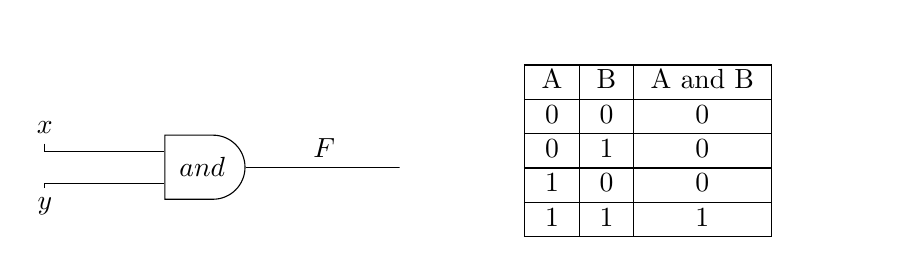
\begin{tikzpicture}
\node (x) at (0, 1) {$x$};
\node (y) at (0, 0) {$y$};
\node[and gate US, draw,logic gate inputs=nnn] at (2,.5) (and) {$and$};
\draw (x)  |- (and.input 1);
\draw (y)  |- (and.input 3);
\draw (and.output) -- ++(2,0) node [midway,anchor=south]{$F$};
\draw[shift={(60:1cm)},xshift=4cm]
node [right,text width=6cm,rounded corners,fill=white,inner sep=1ex]
{
\begin{center}
  \begin{tabular}{ | c | c | c | }
    \hline
    A & B & A and B \\ \hline
    0 & 0 & 0 \\ \hline
    0 & 1 & 0 \\ \hline
    1 & 0 & 0 \\ \hline
    1 & 1 & 1 \\
    \hline
  \end{tabular}
\end{center}
};
\end{tikzpicture}
%\draw (x)  -- ++(.5,0) |- (and.input 1);
%\draw (y)  -- ++(.5,0) |- (and.input 3);

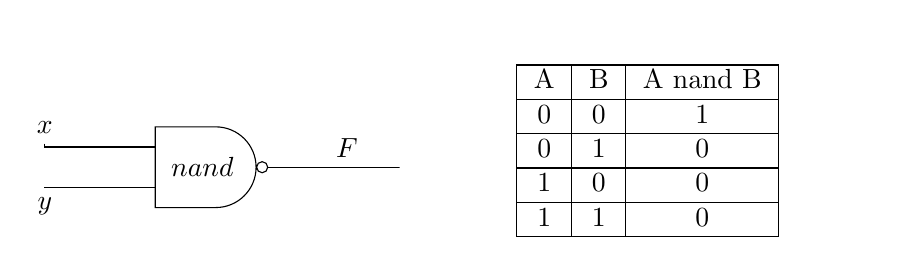
\begin{tikzpicture}
\node (x) at (0, 1) {$x$};
\node (y) at (0, 0) {$y$};
\node[nand gate US, draw,logic gate inputs=nnn] at (2,.5) (nand) {$nand$};
\draw (x)  |- (nand.input 1);
\draw (y)  |- (nand.input 3);
\draw (nand.output) -- ++(2,0) node [midway,anchor=south]{$F$};
\draw[shift={(60:1cm)},xshift=4cm]
node [right,text width=6cm,rounded corners,fill=white,inner sep=1ex]
{
\begin{center}
  \begin{tabular}{ | c | c | c | }
    \hline
    A & B & A nand B \\ \hline
    0 & 0 & 1 \\ \hline
    0 & 1 & 0 \\ \hline
    1 & 0 & 0 \\ \hline
    1 & 1 & 0 \\
    \hline
  \end{tabular}
\end{center}
};
\end{tikzpicture}


\begin{tikzpicture}
\node (x) at (0, 0) {$x$};
\node[not gate US, draw] at (2,0) (not) {$not$};
\draw (x)  --  (not.input);
\draw (not.output) -- ++(2,0) node [midway,anchor=south]{$F$};
\draw[shift={(60:1cm)},xshift=4cm,yshift=-.8cm]
node [right,text width=6cm,rounded corners,fill=white,inner sep=1ex]
{
\begin{center}
  \begin{tabular}{ | c | c | }
    \hline
    A  & not A \\ \hline
    0 & 1 \\ \hline
    1 & 0 \\
    \hline
  \end{tabular}
\end{center}
};
\end{tikzpicture}
%\node[nand gate US, draw] at (0,2) (nand) {};
%\node[not gate US, draw] at (0,0) (not) {};


Unfortunately, both AND and NAND are irreversible Boolean operations By that we
mean that from the output value(s) of the gate one can not determine unambiguously the
input values; information gets irreversibly lost  ''during the gate operation''.

We talk about a reversible gate, Boolean function, operation or computation, as one with always enough information in the outputs to deduce the inputs unambiguously. Such operations, gates and computations are crucial for quantum computing because of the reversibility of the evolution in quantum physics. Three reversible gates have turned out to be of special importance : the usual NOT gate (N), CONTROL NOT gate (CN or CNOT or XOR),  CONTROL CONTROL NOT gate (CCN or CCNOT) , also called Toffoli gate In the CN gate $A^{\prime} = A $, i.e  the input A gets through unchanged .


The filled circle on the first wire represents a control in the following sense : if $A = 0$ then $ \otimes $ on the second wire just lets the signal $B$ get through and therefore $ B^{\prime} = B $.
If $A = 1$, then $ \otimes $ 
on the second wire acts as a NOT gate and
$B^{\prime} = \bar{B}$.

In the CCN gate $A^{\prime} = A$ and $B^{\prime} = B$. 
The $ \otimes $ on the last wire acts as a NOT gate but only if $A = B = 1$

\newpage

\begin{center}
	\includegraphics[scale=1]{./reversible.png}
	%\caption{}
\end{center}

\begin{center}
  \begin{tabular}{ | c | c | }
    \hline
    A  & not A \\ \hline
    0 & 1 \\ \hline
    1 & 0 \\
    \hline
  \end{tabular}
\end{center}


\begin{center}
	\includegraphics[scale=1]{./reversible_2.png}
	%\caption{}
\end{center}


\begin{center}
  \begin{tabular}{ | c | c | c | c | }
  \hline
    A & B & $A^{\prime}$ & $B^{\prime}$ \\ \hline
    0 & 0 & 0 & 0 \\ \hline
    0 & 1 & 0 & 1 \\ \hline
    1 & 0 & 1 & 1 \\ \hline
    1 & 1 & 1 & 0 \\
    \hline
  \end{tabular}
\end{center}

\newpage

\begin{center}
	\includegraphics[scale=1]{./reversible_3.png}
	%\caption{}
\end{center}

\begin{center}
  \begin{tabular}{ | c | c | c | c | c | c | }
  \hline
    A & B & C & $A^{\prime}$ & $B^{\prime}$ & $C^{\prime}$ \\ \hline
    0 & 0 & 0 & 0 & 0 & 0 \\ \hline
    0 & 0 & 1 & 0 & 0 & 1 \\ \hline
    0 & 1 & 0 & 0 & 1 & 0 \\ \hline
    0 & 1 & 1 & 0 & 1 & 1 \\ \hline
    1 & 0 & 0 & 1 & 0 & 0 \\ \hline
    1 & 0 & 1 & 1 & 0 & 1 \\ \hline
    1 & 1 & 0 & 1 & 1 & 1 \\ \hline
    1 & 1 & 1 & 1 & 1 & 0 \\
    \hline
  \end{tabular}
\end{center}


\chapter{Elements}


\section{Introduction}

The basic elements of quantum computing are easy to identify :
quantum bits, quantum
registers, quantum gates and quantum networks.  However, at this 
point ananalogy with
classical computing ends . Quantum bits, registers, gates and 
networks are very different ,
have other properties and larger power than their classical 
counterparts .


A quantum bit can be in any state within an infinite set of 
states. A quantum register
of n quantum bits can be, at the same time,  in any of the 
infinitely many superpositions
of
$2^{n}$
basis states. The parallelism a quantum register can exhibit 
is striking.  The key new
feature is that a quantum register can be in an entangled 
state. On one side,  entangled
states with their non-locality features are a hallmark of 
quantum mechanics. On the other
side, quantum entanglement is an important resource of 
quantum information processing .
There is a larger variety of quantum gates than of classical 
gates  There are already
infinitely many one-input/output quantum gates. In addition  
almost any two-input/output
quantum gate is universal. A simple two-input/output gate 
together with one input rotation
gates form a set of universal gates .

The aim of the chapter is to learn :

\begin{enumerate}
	\item the basic concepts concerning quantum bits and registers
	\item the concept of quantum entanglement and the examples of its power
	\item the basic examples of quantum gates and of quantum circuits
	\item some examples of universal quantum gates and a method to show universality of quantum gates
	\item the basic quantum arithmetical circuits
	\item the concept of quantum superoperator circuits
\end{enumerate}


\section{Quantum Bits and Registers}

Four key problems of quantum information processing are: how to represent, how to store,
how to transmit and how to manipulate quantum information. Two key elements to deal with these problems are quantum bits and quantum registers.


\subsection{Qubits}

Let $S$ be a two dimensional quantum system with two orthonormal states, denoted $\ket{0}$ and $\ket{1}$ , that can be considered as forming a natural, or standard, or preferred, basis of $S$.


\subsubsection{Definition of Qubit}
A qubit (quantum bit) is a quantum state
$$
\ket{\phi} = \alpha\ket{0} + \beta\ket{1}
$$

where $\alpha, \beta \in C$ and $|\alpha|^{2} + |\beta|^{2} = 1$


\subsection{Qubit representations by energy levels of an electron}

\begin{center}
	\includegraphics[scale=.8]{./qubit_1.png}
	%\caption{}
\end{center}


\begin{center}
	\includegraphics[scale=.8]{./qubit_2.png}
	%\caption{}
\end{center}


There are many ways to realize qubits, there are many interesting/important two 
dimensional quantum systems known in physics.  For example,  by the polarization of a
photon or by the ground (n=1) and excited (n=2) states of an electron in the hydrogen
atom. One of the most often and best-explored two-level quantum systems is that of spin-$\frac{1}{2}$ particles with two basis states: spin-up (notation $\ket{\uparrow}$ or $\ket{0}$ ) and spin-down
(notation$\ket{\downarrow}$ or $\ket{1}$ ) 



From the implementation point of view the most promising candidates for qubits are so
far photons, trapped ions and spins of atomic nuclei.

States $\ket{0}$ and $\ket{1}$ of a qubit 
can be seen, and are often referred to, as representing
classical states (bits).
The main difference between classical bits and qubits is that 
while a classical bit can be set up only to one of the two 
states, namely 0 or 1 a qubit can take any
quantum linear superposition of $\ket{0}$ and $\ket{1}$,
i.e: in principle can be in any of uncountably
many states. This means that a large, even infinite, amount of information could potentially
be encoded in amplitudes of a single qubit by appropriately choosing $\alpha$ and  $\beta$

One way to represent states of qubits geometrically is as points on the surface of a
unit Riemann sphere, where North and South poles correspond to the basis states (that correspond to bits).
Qubits can be represented also by points on a Bloch-sphere , using the
spherical coordinate system .
This representation is based on the fact that any qubit can be
represented as $\cos{\frac{\theta}{2}}\ket{0} + e^{i\phi}\sin{\frac{\theta}{2}}\ket{1}$



\begin{center}
	\includegraphics[scale=.6]{./sphere1.png}
	%\caption{}
\end{center}



\section{Qubit evolution}

Any quantum evolution of a qubit, or any quantum operation on a qubit is described, as
already mentioned by a unitary matrix :

$$
A = 
\begin{pmatrix}
a & b\\
c & d 
\end{pmatrix}	
$$


which transforms any qubit state
$\alpha\ket{0} + \beta\ket{1}$
into the state
$(a\alpha+b\beta)\ket{0} + (c\alpha+d\beta)\ket{1}$


\section{Two-qubit registers}

A tensor product of two qubits is called a 2-qubit quantum register,in 2-qubit quantom registers the state $\ket{11}$
 is called singleton

It is usual to represent states of the standard basis in one of the following forms :

$$
\ket{0} = 
\ket{00} =
\begin{pmatrix}
1\\
0\\
0\\
0
\end{pmatrix}
\qquad
\ket{1} = 
\ket{01} =
\begin{pmatrix}
0\\
1\\
0\\
0
\end{pmatrix}
$$

$$
\ket{2} = 
\ket{10} =
\begin{pmatrix}
0\\
0\\
1\\
0
\end{pmatrix}
\qquad
\ket{3} = 
\ket{11} =
\begin{pmatrix}
0\\
0\\
0\\
1
\end{pmatrix}
$$


A general state of a 2-qubit quantum register has the form

$$
\ket{\psi} = \alpha_{00}\ket{00} + \alpha_{01}\ket{01} + \alpha_{10}\ket{10} + \alpha_{11}\ket{11} 
$$

where $|\alpha_{00}|^{2}+ |\alpha_{01}|^{2} +|\alpha_{10}|^{2} +|\alpha_{11}|^{2} = 1$



\section{Quantom registers}


\section{Quantom gates}

The gates for basic Boolean reversible operations NOT, CNOT, and CCNOT can be
described also using a notation for registers as follows :


\begin{eqnarray*}
\textbf{NOT}&:&\ket{a} \to \ket{\bar{a}}\\
\textbf{XOR = CNOT} &:&  \ket{a , b} \to \ket{a ,  a \oplus b} \\
\textbf{CCNOT} &:& \ket{a , b, c} \to \ket{a , b ,  ( a \wedge b ) \oplus c}
\end{eqnarray*}


\end{document}